\tikzstyle{s} = [rectangle, rounded corners, minimum width=2cm, text width=2cm, minimum height=1cm, text centered, draw=black]
\tikzstyle{arrow} = [thick,->,>=stealth]
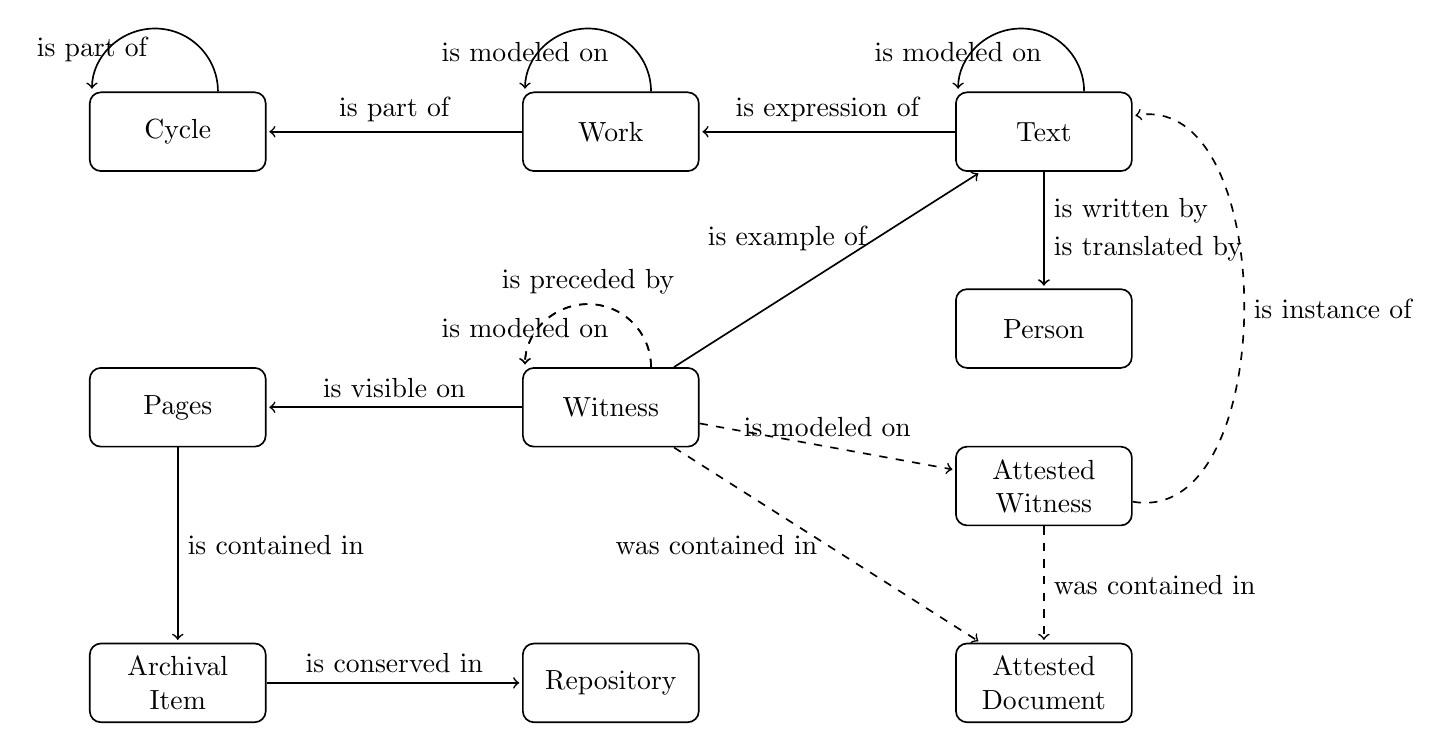
\begin{tikzpicture}[-,shorten >=1pt,auto,node distance=2.5cm,semithick]
\tikzstyle{every state}=[fill=red,draw=none,text=white]

\node[s] (cycle) [] {Cycle};
\node[s] (work) [right of=cycle, xshift=3cm] {Work};
\node[s] (text) [right of=work, xshift=3cm] {Text};

\node[s] (person) [below of=text] {Person};

\node[s] (attestedWitness) [below of=person, yshift=0.5cm] {Attested Witness};

\node[s] (witness) [below of=work, yshift=-1cm] {Witness};

\node[s] (pages) [left of=witness, xshift=-3cm] {Pages};

\node[s] (item) [below of=pages, yshift=-1cm] {Archival Item};

\node[s] (repo) [right of=item, xshift=3cm] {Repository};

\node[s] (document) [right of=repo, xshift=3cm] {Attested Document};

% \draw[dashed, ->] (witness.-45) arc (200:475:8mm) 
%   node[pos=0.5, below] () {is preceded by};
\draw[dashed, ->] (witness.45) arc (0:180:8mm)
  node[above, pos=0.5] () {is preceded by};
\draw[dashed, ->] (witness.45) arc (0:180:8mm)
  node[above, yshift=0.25cm] () {is modeled on};
\draw[->] (cycle.45) arc (0:180:8mm) 
  node[above, yshift=0.25cm] () {is part of};
\draw[->] (work.45) arc (0:180:8mm) 
  node[above, yshift=0.25cm] () {is modeled on};
\draw[->] (work) -- (cycle)
  node[pos=0.5, above] () {is part of};
\draw[->] (text) -- (work)
  node[pos=0.5, above] () {is expression of};
\draw[->] (witness) -- (text)
  node[pos=0.66, left] () {is example of};
\draw[dashed,->] (witness) -- (document)
  node[pos=0.5, left] () {was contained in};
\draw[->] (pages) -- (item)
  node[pos=0.5, right] () {is contained in};
\draw[->] (witness) -- (pages)
  node[pos=0.5, above] () {is visible on};
\draw[->] (item) -- (repo)
  node[pos=0.5, above] () {is conserved in};
\draw[->] (text.45) arc (0:180:8mm) 
  node[yshift=0.25cm, above] () {is modeled on};
\draw[->] (text) -- (person)
  node[pos=0.66, right] {is translated by};
\draw[->] (text) -- (person)
  node[pos=0.33, right] {is written by};
\draw[dashed, ->] (witness) -- (attestedWitness)
  node[pos=0.5, above] {is modeled on};
\draw[dashed, ->] (attestedWitness) -- (document)
  node[pos=0.5, right] {was contained in};

\path[every node]
  (attestedWitness) edge[dashed, ->, bend right=100] node [pos=0.5, right] {is instance of} (text)
  ;

\end{tikzpicture}